\documentclass[journal,10pt,twocolumn]{article}
\usepackage{graphicx}
\usepackage[margin=0.5in]{geometry}
\usepackage{amsmath}
\usepackage{array}
\usepackage{booktabs}
\usepackage{listings}
\providecommand{\norm}[1]{\left\lVert#1\right\rVert}
\providecommand{\abs}[1]{\left\vert#1\right\vert}
\usepackage{enumerate}
\let\vec\mathbf
\newcommand{\myvec}[1]{\ensuremath{\begin{pmatrix}#1\end{pmatrix}}}
\newcommand{\mydet}[1]{\ensuremath{\begin{vmatrix}#1\end{vmatrix}}}
\providecommand{\brak}[1]{\ensuremath{\left(#1\right)}}
\lstset{
frame=single,
breaklines=true,
columns=fullflexible
}
\title{\textbf{Matrix Assignment}}
\author{Mannava Venkatasai}
\date{September 2022}
\begin{document}
\maketitle
\raggedright \textbf{Problem Statement} :\vspace{3mm} \\ Find the maximum and minimum values of the function : f(x) = 9$x^2$+12$x$+2 
\section*{Solution}
\begin{figure}[h]
\centering
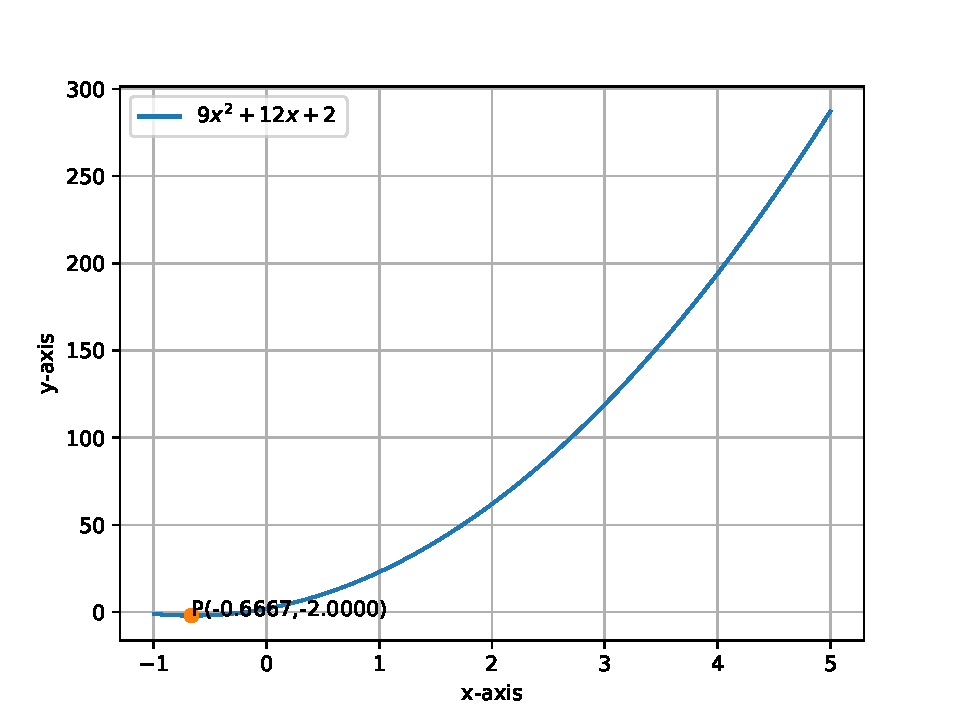
\includegraphics[width=1\columnwidth]{opt2.pdf}
	\caption{f(x) = 9$x^2$+12x+2}
\label{fig:Curve}
\end{figure}
\section*{Solution}
\subsection*{Part 1}
Given the function:
\begin{align}
f(x) = 9x^2+12x+2 
\end{align}
This can be written as :
\begin{align}
f(x) = (3x+2)^2-2 
\end{align}
\begin{align}
(3x+2)^2\ge 0
\end{align}
so
\begin{align}
f(x) \ge-2 
\end{align}
The maximum value of f(x) is $\infty$ \vspace{5mm} \\
Hence the function having only minimum value \\
The minimum value is caluculated by using gradient descent method.
\begin{align}
        x_{n+1} &= x_n - \alpha \nabla f(x_n) \\
        \implies x_{n+1} &= x_n - \alpha \brak{18x_n+12}
\end{align}
where \\
\begin{enumerate}
\item $\alpha$ = 0.001
\item $x_{n+1}$ is current value
\item $x_{n}$ is previous value
\item precession = 0.00000001
\item maximum iterations = 100000000
\end{enumerate}
The minimum values obtained from the python code \vspace{5mm}\\
The given function has minimum value at
\begin{align} 
x=\frac{-2}{3} \\
Minimum&=-2
\end{align}
\end{document}
